\documentclass[17pt]{beamer}
%\documentclass[handout]{beamer} %Makes Handouts
\usetheme{Singapore} %Gray with fade at top
\useoutertheme[subsection=false]{miniframes} %Supppress subsection in header
\useinnertheme{rectangles} %Itemize/Enumerate boxes
\usecolortheme{seagull} %Color theme
\usecolortheme{rose} %Inner color theme

\definecolor{light-gray}{gray}{0.75}
\definecolor{dark-gray}{gray}{0.55}
\setbeamercolor{item}{fg=light-gray}
\setbeamercolor{enumerate item}{fg=dark-gray}

\setbeamertemplate{navigation symbols}{}
\setbeamertemplate{mini frames}{}
%\setbeamercovered{dynamics}
\setbeamerfont*{title}{size=\Large,series=\bfseries}
\setbeamerfont{footnote}{size=\tiny}

%\setbeameroption{notes on second screen} %Dual-Screen Notes
%\setbeameroption{show only notes} %Notes Output

\setbeamertemplate{frametitle}{\vspace{.5em}\bfseries\insertframetitle}
\newcommand{\heading}[1]{\noindent \textbf{#1}\\ \vspace{1em}}
\newcommand{\questions}{\frame{{\large Questions?}}}

\usepackage{bbding,color,multirow,times,ccaption,tabularx,graphicx,verbatim,booktabs}
\usepackage{colortbl} %Table overlays
\usepackage[english]{babel}
\usepackage[latin1]{inputenc}
\usepackage[T1]{fontenc}
\usepackage{lmodern}
\usepackage{alltt}

\usepackage{tikz}
\usetikzlibrary{shapes,arrows,decorations.pathreplacing,calc}


\author[]{Thomas J. Leeper}
\institute{
  Government Department\\London School of Economics and Political Science
}

\usepackage{multirow}

\setbeamertemplate{headline}
 {%
  \begin{beamercolorbox}{section in head/foot}
  \insertsectionnavigationhorizontal{\textwidth}{}{}
  \end{beamercolorbox}%
}

\title{Session IV\\Sources of Heterogeneity}

\date[]{}

\begin{document}

\frame{\titlepage}

\frame{\tableofcontents}

\section[Other Designs]{Other Survey Experimental Designs}
\frame{\tableofcontents[currentsection]}

\frame{

\frametitle{{\normalsize Beyond One-shot Designs}}

\small

\begin{itemize}\itemsep0.5em
\item Surveys can be used as a measurement instrument for a field treatment or a manipulation applied in a different survey panel wave
	\begin{enumerate}\footnotesize
	\item Measure effect duration in two-wave panel
	\item Solicit pre-treatment outcome measures in a two-wave panel
	\item Measure effects of field treatment in post-test only design
	\item Randomly encourage field treatment in pre-test and measure effects in post-test
	\end{enumerate}
\item<2-> Problems? Compliance \& nonresponse
\end{itemize}

}


\frame{

\frametitle{{\normalsize I. Effect Duration}}

\begin{itemize}\itemsep0.5em
\item Use a two- (or more-) wave panel to measure duration of effects
	\begin{itemize}
	\item T1: Treatment and outcome measurement
	\item T2+: Outcome measurement
	\end{itemize}
\item Two main concerns
	\begin{itemize}
	\item Attrition
	\item Panel conditioning
	\end{itemize}
\end{itemize}

}

\frame{

\frametitle{{\normalsize II. Within-Subjects Designs}}

\small

\begin{itemize}
\item Estimate treatment effects as a difference-in-differences
\item Instead of using the post-treatment mean-difference in $Y$ to estimate the causal effect, use the difference in pre-post differences for the two groups:
	\begin{align*}
	(\hat{Y}_{0,t+1} - \hat{Y}_{0,t}) - (\hat{Y}_{j,t+1} - \hat{Y}_{j,t})
	\end{align*}
\item<2-> Advantageous because variance for paired samples decreases as correlation between $t_0$ and $t_1$ observations increases
\end{itemize}

}


\frame{
	\begin{center}
	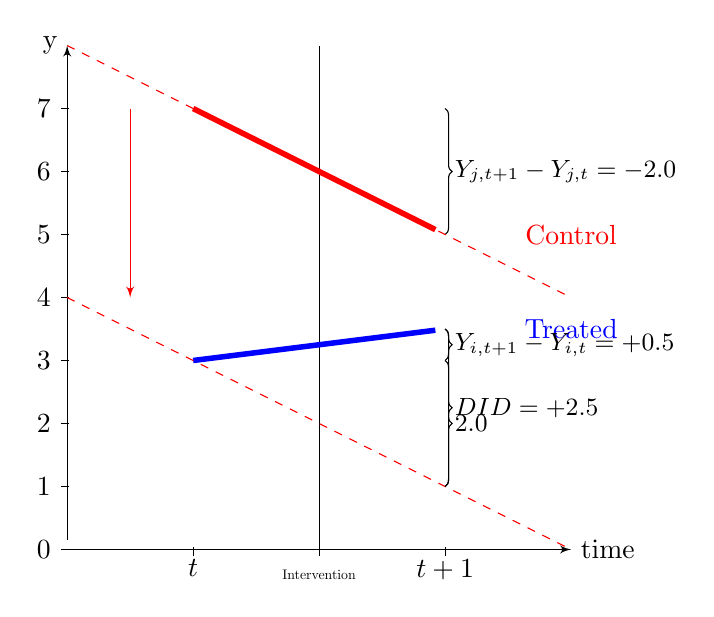
\begin{tikzpicture}[>=latex', scale=0.8]
        \draw[->] (0,0) node (origin) {}  -- (8,0) node[right] (xaxis) {time};
        \draw[->] (origin) -- (0,8) node[left] (yaxis) {y};
        % x ticks
        \foreach \x in {2,4,6}
        	\draw (\x,1pt) -- (\x,-3pt) node[anchor=north] {};
        \draw (2,0) node[below] (before) {$t$};
        \draw (6,0) node[below] (after) {$t+1$};
        \draw (4,-0.25) node[below, scale=0.5] (IV) {Intervention};
        % y ticks
        \foreach \y in {0,...,7}
             \draw (1pt,\y) -- (-3pt,\y) node[anchor=east] {$\y$};
        % intervention
        \draw (4,0) -- (4,8);

        % line
        \draw<2-> (6,3.5) node (tr) {};
        \draw<3-> (6,5) node (ctrl) {};
        \draw<2-3>[blue] (8,3.5) node (trlab) {Treated};
        \draw<3-3>[red] (8,5) node (ctrllab) {Control};        
        \draw<2->[blue, line width=2pt] (2,3) -- (tr);
        \draw<3->[red, line width=2pt] (2,7) -- (ctrl);
        
        % diffs
        \draw<4-6>[right,decorate,decoration={brace,mirror}] 
        	(6,3) -- (6,3.5) node[right, pos=0.5] (idiff) {\small $Y_{i,t+1} - Y_{i,t} = +0.5$};
        \draw<4-6>[right,decorate,decoration={brace}] 
            (6,7) -- (6,5) node[right, pos=0.5] (jdiff) {\small $Y_{j,t+1} - Y_{j,t} = -2.0$};
        
        % trends
        \draw<5-6>[red,->] (1,7) -- (1,4);
        \draw<5->[red, dashed] (0,8) -- (8,4);
        \draw<5->[red, dashed] (0,4) -- (8,0);
        \draw<6>[right,decorate,decoration={brace}] 
            (6,3) -- (6,1) node[right, pos=0.5] (idiff2) {\small $2.0$};
        \draw<7>[right,decorate,decoration={brace}] 
            (6,3.5) -- (6,1) node[right, pos=0.5] (idiff2) {\small $DID = +2.5$};
                        
        
    \end{tikzpicture}
    \end{center}
}


\frame{

	\frametitle{{\normalsize Threats to Validity}}
	
	\small
	
	As soon as time comes into play, we have to worry about threats to validity.\footnote{Shadish, Cook, and Campbell (2002)}
	
	\begin{enumerate}
	\item<2-> History (simultaneous cause)
	\item<3-> Maturation (time trends)
	\item<4-> Testing (observation changes respondents)
	\item<5-> Instrumentation (changing operationalization)
	\item<6-> Instability (measurement error)
	\item<7-> Attrition
	\end{enumerate}
}






\frame{

\frametitle{{\normalsize III. Randomized Field Treatment}}

\small

\begin{itemize}\itemsep-0.2em
\item Examples:
	\begin{enumerate}
	\item<2-> Citizens randomly sent a letter by post encouraging them to reduce water usage
	\item<3-> Different local media markets randomly assigned to receive different advertising
	\end{enumerate}
\item<4-> Survey is used to measure outcomes, when treatment assignment is already known
\item<5-> Issues
	\begin{itemize}
	\item<6-> Nonresponse
	\item<6-> Noncompliance
	\end{itemize}
\end{itemize}

}

\frame{

\frametitle{{\normalsize IV. Treatment Encouragement}}

\small

\begin{itemize}\itemsep-0.2em
\item Design:
	\begin{itemize}
	\item T1: Encourage treatment
	\item T2: Measure effects
	\end{itemize}
\item Examples:
	\begin{enumerate}
	\item Albertson and Lawrence
	\end{enumerate}
\item<2-> Issues
	\begin{itemize}
	\item<3-> Nonresponse
	\item<3-> Noncompliance
	\end{itemize}
\end{itemize}

}


\frame{

\frametitle{{\normalsize Treatment Noncompliance}}

\begin{itemize}\itemsep0.5em
\item Definition:\\{\small ``when subjects who were assigned to receive the treatment go untreated or when subjects assigned to the control group are treated'' \footnote{Gerber \& Green. 2012. \textit{Field Experiments}, p.132.}}
\item<2-> Several strategies
	\begin{itemize}
	\item ``As treated'' analysis
	\item ``Intention to treat'' analysis
	\item Estimate a LATE
	\end{itemize}
\end{itemize}

}

\frame{
\frametitle{{\normalsize Analyzing Noncompliance}}

\small

\begin{itemize}\itemsep0.5em
\item If noncompliance only occurs in one group, it is \textit{asymmetric} or \textit{one-sided}
\item We can ignore non-compliance and analyze the ``intention to treat'' effect, which will underestimate our effects because some people were not treated as assigned: $ITT = \overline{Y}_1 - \overline{Y}_0$
\item<2-> We can use ``instrumental variables'' to estimate the ``local average treatment effect'' (LATE) for those that complied with treatment: $LATE = \frac{ITT}{\% Compliant}$
\end{itemize}
}

\frame{
	\frametitle{{\large Local Average Treatment Effect}}
	\small
	\begin{itemize}\itemsep0.2em
	\item IV estimate is \textit{local} to the variation in $X$ that is due to variation in $D$
	\item This matters if effects are \textit{heterogeneous}
	\item LATE is effect for those who \textit{comply}
	\item Four subpopulations:
		\begin{itemize}\footnotesize
		\item Compliers: $X = 1$ only if $D = 1$
		\item Always-takers: $X = 1$ regardless of $D$
		\item Never-takers: $X = 0$ regardless of $D$
		\item Defiers: $X = 1$ only if $D = 0$
		\end{itemize}
	\item Exclusion restriction! Monotonicity!
	\end{itemize}
}

\questions


\section{Attention and Satisficing}
\frame{\tableofcontents[currentsection]}

\frame{

How should we deal with respondents that appear to not be paying attention, not ``taking'' the treatment, or not responding to outcome measures?

\begin{enumerate}
\item Keep them
\item Throw them away
\end{enumerate}

}

\frame{

\frametitle{Best Practice: Protocol}

\begin{itemize}\itemsep0.5em
\item Excluding respondents based on survey behavior is one of the easiest ways to ``p-hack'' an experimental dataset
	\begin{itemize}
	\item Inattention, satisficing, etc. will tend to reduce the size of the SATE
	\end{itemize}
\item So regardless of how you handle these respondents, these should be decisions that are made \textit{pre-analysis}
\end{itemize}

}


\frame[label=exclusion]{

\frametitle{{\normalsize When are you excluding participants?}}

    \begin{columns}[T]
    \begin{column}[T]{5cm}
        \begin{block}{\rule[-0.6ex]{0pt}{2.5ex}Pre-Treatment}
            \begin{itemize}\itemsep0.2em
                \item<2-> \hyperlink{satisficing}{Satisficing behaviors}
                \item<3-> Inattention
                \item<4-> Covariate-based selection
                \item<5-> Pretreated
            \end{itemize}
        \end{block}
    \end{column}
    \begin{column}[T]{5cm}
        \begin{block}{\rule[-0.6ex]{0pt}{2.5ex}Post-Treatment}
            \begin{itemize}\itemsep0.5em
                \item<6-> Speeding on treatment
                \item<7-> ``Failing'' a manipulation check
                \item<8-> Drop-off
            \end{itemize}
        \end{block}
    \end{column}
    \end{columns}

}


\frame{

\frametitle{Pre-Treatment Exclusion}

\begin{itemize}\itemsep0.5em
\item This is totally fine from a causal inference perspective
\item<2-> Advantages:
	\begin{itemize}
	\item Focused on engaged respondents
	\item Likely increase impact of treatment
	\end{itemize}
\item<3-> Disadvantages:
	\begin{itemize}
	\item Changing definition of sample (and thus population)
	\end{itemize}
\end{itemize}

}




\frame{

\frametitle{Post-Treatment Exclusion}

This is much more problematic because it involves controlling for a \textit{post-treatment} variable

}

\frame<1-3>[label=posttreatment]{

\begin{center}
\begin{tikzpicture}[>=latex',circ/.style={draw, shape=circle, node distance=5cm, line width=1.5pt}]
    \draw (0,0) node[left, text width=3cm, align=center] (X) {Information};
    \draw (5,0) node[right, text width=2cm, align=center] (Y) {Opinion};
    \draw<1-3>[->] (X) -- (Y);
    \draw[->] (4,-4) node[below, text width=3cm, align=center] (E) {Etc.} -- (Y);
	\draw<2-> (1,-2) node[text width=3cm, align=center] (M) {Manipulation Check};
	\draw<2-4>[->,thick,red] (X) -- (M);
    \draw<2-4>[->,thick,red] (M) -- (Y);
    \draw<3>[->] (E) -- (M);
\end{tikzpicture}
\end{center}

\small 
\only<2>{Risk that estimate of $\beta_1$ is diminished because effect is being carried through the manipulation check.}
\only<3>{Introduction of ``collider bias'' wherein values of the manipulation check are affected by other factors.}
}





\frame[label=posttreatment2]{

\frametitle{Post-Treatment Exclusion}

\small

\begin{itemize}\itemsep0.5em
\item Any post-treatment exclusion is problematic and should be avoided
\item<2-> Can estimate a LATE
	\begin{itemize}\footnotesize
	\item Interpretation: Effect of manipulation check among those whose value of the check can be changed by the treatment manipulation
	\end{itemize}
\item<3-> Non-response or attrition is the same as researcher-imposed exclusion
	\begin{itemize}\footnotesize
	\item Not problematic if MCAR
	\item Nothing really to be done if caused by treatment
	\end{itemize}
\end{itemize}

}

\againframe<3-4>{posttreatment}

\againframe<2->{posttreatment2}


\questions

\section[Moderators]{Moderators and Effect Heterogeneity}
\frame{\tableofcontents[currentsection]}


\frame{

If we think there might be effect heterogeneity, what can we do?

\begin{itemize}
\item Best solution: manipulate the moderator
\item Next best: block on the moderator
\item Least best: post-hoc exploratory approaches
\end{itemize}
}




\subsection{Manipulate the Moderator}


\frame{

Simply: Manipulating the moderator variable is the best way to estimate a heterogeneous effect!

\vspace{1em}

Why is this true?

}


\begin{frame}
\begin{center}
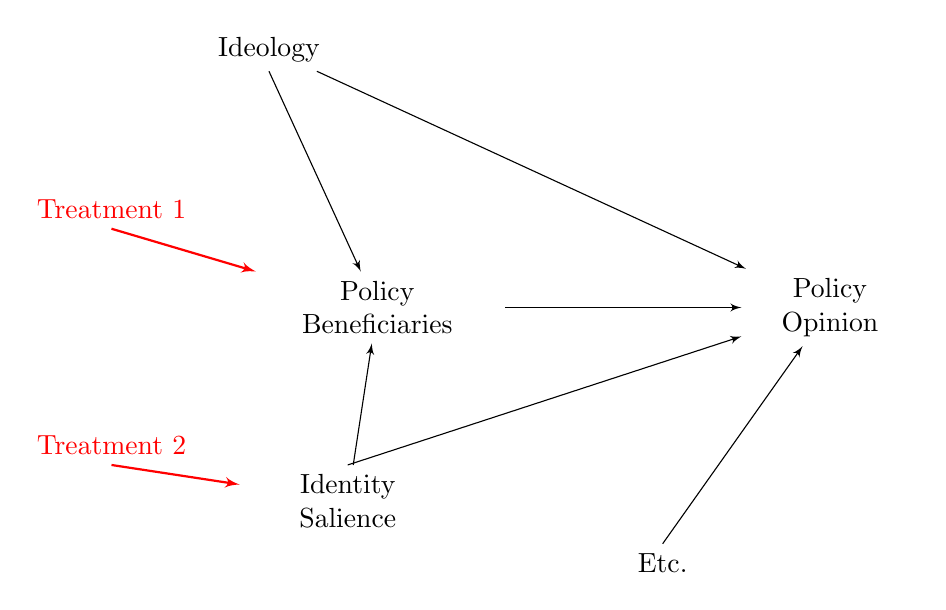
\begin{tikzpicture}[>=latex',circ/.style={draw, shape=circle, node distance=5cm, line width=1.5pt}]
    \draw (0,0) node[left, text width=3cm, align=center] (X) {Policy\\Beneficiaries};
    \draw[->] (X) -- (3,0) node[right, text width=2cm, align=center] (Y) {Policy\\Opinion};
    \draw[->] (-3,3) node[above] (Z) {Ideology} -- (X);
    \draw[->] (Z) -- (Y);
    \draw[->] (2,-3) node[below, text width=3cm, align=center] (E) {Etc.} -- (Y);
    \draw[->] (-2, -2) node[below, text width=2.5cm, align=center] (W) {Identity Salience} -- (Y);
    \draw[->] (W) -- (X);
    \draw<2->[->,thick,red] (-5,1) node[above] (T1) {Treatment 1} -- (X);
    \draw<2->[->,thick,red] (-5,-2) node[above] (T1) {Treatment 2} -- (W);
\end{tikzpicture}
\end{center}
\end{frame}



\frame{
	\frametitle{{\normalsize Ex. Question-as-treatment\footnote{Transue. 2007. ``Identity Salience, Identity Acceptance, and Racial Policy Attitudes: {American} National Identity as a Uniting Force.'' \textit{American Journal of Political Science} 51(1): 78--91.}}}
	

\begin{itemize}
\item \only<1,3>{How close do you feel to your ethnic or racial group?}\only<2,4>{How close do you feel to other Americans?}
\item \only<1-2>{Some people have said that taxes need to be raised to take care of pressing national needs. How willing would you be to have your taxes raised to improve education in public schools?}\only<3-4>{Some people have said that taxes need to be raised to take care of pressing national needs. How willing would you be to have your taxes raised to improve educational opportunities for minorities?}
\end{itemize}
	
}


\frame{

\frametitle{2x2 Factorial Design}

\only<1>{
\begin{center}
\begin{tabular}{lr}
Condition &  \\ \midrule
Educ. for Minorities & $Y_1$ \\
Schools & $Y_0$ \\ \bottomrule
\end{tabular}
\end{center}
}

\only<2>{
\begin{center}
\begin{tabular}{lrr}
Condition & Americans & Own Race \\ \midrule
Educ. for Minorities & $Y_{1,0}$ & $Y_{1,1}$ \\
Schools & $Y_{0,0}$ & $Y_{0,1}$ \\ \bottomrule
\end{tabular}
\end{center}
}

}


\frame{

\frametitle{Two ways to estimate this}

Dummy variable regression:

$Y = \beta_0 + \beta_1 X_{0,1} + \beta_2 X_{1,0} + \beta_3 X_{1,1} + \epsilon$

\vspace{1em}

Interaction effect:

$Y = \beta_0 + \beta_1 X1_{1} + \beta_2 X2_{1} + \beta_3 X1_1 * X2_1 + \epsilon$

}


\frame<1>[label=factorialconsiderations]{

\frametitle{Considerations}

\begin{itemize}\itemsep0.5em
\item Need to have hypotheses about heterogeneity a priori
\item Factorial designs can quickly become unwieldy and expensive
\item<2-> Need to consider what CATEs are of theoretical interest
	\begin{itemize}
	\item Treatment--control
	\item Treatment--treatment
	\end{itemize}
\end{itemize}

}

\frame{

\frametitle{Probably obvious, but\dots}

\footnotesize

\begin{center}
\begin{tabular}{cccc}
Factors & Conditions per factor & Total Conditions & $n$ \\ \midrule
1 & 2 & 2 & 400 \\ 
1 & 3 & 3 & 600 \\
1 & 4 & 4 & 800 \\
2 & 2 & 4 & 800 \\
2 & 3 & 6 & 1200 \\
2 & 4 & 8 & 1600 \\
3 & 3 & 9 & 1800 \\
3 & 4 & 12 & 2400 \\
4 & 4 & 16 & 3200 \\ \bottomrule
\end{tabular}
\end{center}

{\footnotesize Assumes power to detect a relatively small effect, but no consideration of multiple comparisons.}

}

\againframe{factorialconsiderations}

% marginal effects of factors are marginal across the set of levels of the other factors; if those factors aren't complete, then external validity problem


\questions


\frame{

\frametitle{Conjoint Designs I}

\small

\begin{itemize}
\item ``Classic vignettes'' taken to an extreme
	\begin{itemize}
	\item Address heterogeneity w/r/t SU\textbf{T}O
	\end{itemize}
\item Example: Judge whether to admit an immigrant to your country
\item<2-> Respondents see a series of vignettes that are fully randomized along any number of dimensions
	\begin{itemize}\footnotesize
	\item Sex, Education, Language proficiency, etc.
	\end{itemize}
\item<3-> Outcome is judgment (binary or rating scale)
\end{itemize}

}

\frame{

\frametitle{Conjoint Designs II}

Why is this useful?

\begin{itemize}\itemsep0.5em
	\item Understand complex decision-making
	\item Within-subjects comparisons
	\item Heterogeneous effects across versions of treatment
	\item Pilot testing: Sensitivity of design to specification of \textit{compound} vignette
\end{itemize}

}


\frame{
\begin{center}
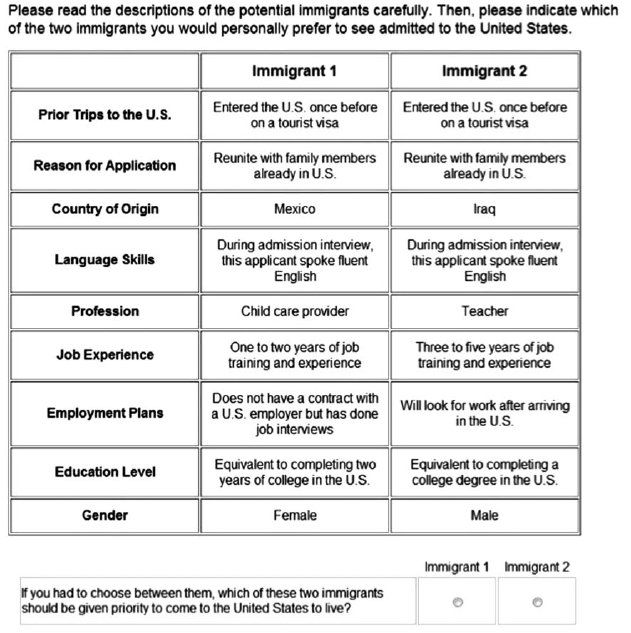
\includegraphics[height=\textheight]{images/conjoint1}
\end{center}
}

\frame{
\begin{center}
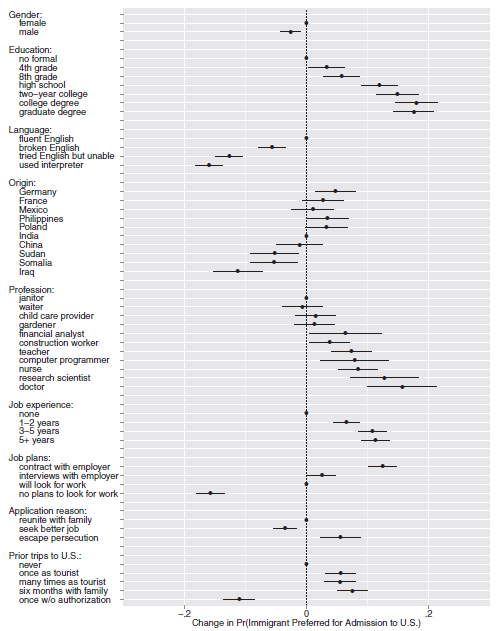
\includegraphics[width=\textwidth]{images/conjoint2}
\end{center}
}

\frame{

\frametitle{Conjoint Designs III}


\begin{itemize}\itemsep0.5em
\item<2-> As long as profiles are randomized, this is just a complex factorial design where we can estimate \textit{marginal effect} of each attribute
	\begin{itemize}\footnotesize
	\item Treatment--control SATE, conditional on all other randomized factors
	\end{itemize}
\item<3-> Assumptions:
	\begin{itemize}\footnotesize
	\item Fully randomized profiles
	\item No ``carry-over'' effects
	\item No profile order effects
	\end{itemize}
\end{itemize}

}

\questions



\frame{

\frametitle{Activity!}

\begin{itemize}\itemsep0.5em
\item Work in groups of 2--3
\item Consider a research question of interest to you
	\begin{itemize}\footnotesize
	\item Opinions on policies
	\item Product purchasing decisions
	\item Information selection
	\item Attitudes toward out-groups
	\item etc.
	\end{itemize}
\item Try to describe a basic conjoint design
	\begin{itemize}
	\item What is the outcome?
	\item What are the factors/features?
	\end{itemize}
\end{itemize}


}


\subsection{Blocking/Block Randomization}


\frame{

\frametitle{Block Randomization I}

{\small \textbf{Stratification:Sampling::Blocking:Experiments}}

\small

\begin{itemize}\itemsep0.5em
\item<2-> Basic idea: randomization occurs within strata defined before treatment assignment
\item<3-> CATE is estimate for each stratum; aggregated to SATE
\item<4-> Why?
	\begin{itemize}
	\item Eliminate chance imbalances
	\item Optimized for estimating CATEs
	\item More precise SATE estimate
	\end{itemize}
\end{itemize}

}

\begin{frame}[fragile]

\begin{center}
\begin{tabular}{lcccccccc}
Exp. & \multicolumn{4}{c}{Control} & \multicolumn{4}{c}{Treatment} \\ \midrule
1 & M & M & M & M & F & F & F & F \\
2 & M & M & M & F & M & F & F & F \\
3 & M & M & F & F & M & M & F & F \\
4 & M & F & F & F & M & M & M & F \\
5 & F & F & F & F & M & M & M & M \\ \bottomrule
\end{tabular}
\end{center}


{\scriptsize
\begin{verbatim}
# population of men and women
pop <- rep(c("Male", "Female"), each = 4)

# randomly assign into treatment and control
split(sample(pop, 8, FALSE), c(rep(0,4), rep(1,4)))
\end{verbatim}
}

\end{frame}

\frame{

\begin{center}

\begin{tabular}{rrrr}
Obs. & $X_{1i}$ & $X_{2i}$ & $D_i$ \\ \midrule
1 & Male & Old & 0 \\
2 & Male & Old & 1 \\  \midrule
3 & Male & Young & 1 \\
4 & Male & Young & 0 \\ \midrule
5 & Female & Old & 1 \\
6 & Female & Old & 0 \\ \midrule
7 & Female & Young & 0 \\
8 & Female & Young & 1 \\ \bottomrule
\end{tabular}
\end{center}

}

\frame[label=blocking2]{

\frametitle{Block Randomization II}

\begin{itemize}
\item Blocking ensures ignorability of all covariates used to construct the blocks
\item Incorporates covariates explicitly into the \textit{design}
\item<2-> When is blocking \textit{statistically} useful?
	\begin{itemize}
	\item<3-> If those covariates affect values of potential outcomes, blocking reduces the variance of the SATE
	\item<4-> Most valuable in small samples
	\item<5-> Not valuable if all blocks have similar potential outcomes
	\end{itemize}
\end{itemize}

}



\frame{

\frametitle{Statistical Properties I}

\small

Complete randomization:\\
$$SATE = \frac{1}{n_1}\sum Y_{1i} - \frac{1}{n_0}\sum Y_{0i}$$

\vspace{2em}

Block randomization:\\
$$SATE_{blocked} = \sum_{1}^{J} \left( \dfrac{n_j}{n} \right)  (\widehat{CATE}_j)$$

}


\frame{

\begin{center}

\begin{tabular}{rrrrrr}
Obs. & $X_{1i}$ & $X_{2i}$ & $D_i$ & $Y_i$ & CATE \\ \midrule
1 & Male & Old & 0 & 5 & \multirow{2}{*}{\onslide<2->{5}} \\
2 & Male & Old & 1 & 10 \\  \midrule
3 & Male & Young & 1 & 4 & \multirow{2}{*}{\onslide<3->{3}} \\
4 & Male & Young & 0 & 1 \\ \midrule
5 & Female & Old & 1 & 6 & \multirow{2}{*}{\onslide<4->{4}} \\
6 & Female & Old & 0 & 2 \\ \midrule
7 & Female & Young & 0 & 6 & \multirow{2}{*}{\onslide<5->{3}} \\
8 & Female & Young & 1 & 9 \\ \bottomrule
\end{tabular}
\end{center}

}

\frame{

\frametitle{SATE Estimation}

\begin{align*}
SATE &= \left(\dfrac{2}{8}*5\right) + \left(\dfrac{2}{8}*3\right) + \left(\dfrac{2}{8}*4\right) + \left(\dfrac{2}{8}*3\right) \\ \vspace{1em}
&= 3.75
\end{align*}

\onslide<2->{The blocked and unblocked estimates are the same here because $Pr(Treatment)$ is constant across blocks and blocks are all the same size.}

}

\frame{

\frametitle{SATE Estimation}

\small

\begin{itemize}
\item We can use weighted regression to estimate this in an OLS framework
\item Weights are the inverse prob. of being treated w/in block
\begin{itemize}
\item Pr(Treated) by block: $p_{ij} = Pr(D_i = 1 | J=j) $
\item Weight (Treated): $ w_{ij} = \dfrac{1}{p_{ij}} $
\item Weight (Control): $ w_{ij} = \dfrac{1}{1-p_{ij}} $
\end{itemize}
\end{itemize}

}


\frame{

\frametitle{Statistical Properties II}

\small

Complete randomization:\\
$$\widehat{SE}_{SATE} = \sqrt{\dfrac{\widehat{Var}(Y_0)}{n_0} + \dfrac{\widehat{Var}(Y_1)}{n_1}}$$

\vspace{1em}

Block randomization:\\
$$\widehat{SE}_{SATE_{blocked}} = \sqrt{\sum_{1}^{J} \left( \dfrac{n_j}{n} \right)^2  \widehat{Var}{(SATE_j)}}$$

\only<2->{When is the blocked design more efficient?}

}


\frame{

\frametitle{Practicalities}

\begin{itemize}\itemsep0.5em
\item Blocked randomization only works in exactly the same situations where stratified sampling works
	\begin{itemize}
	\item Need to observe covariates pre-treatment in order to block on them
	\item Work best in a panel context
	\end{itemize}
\item In a single cross-sectional design that might be challenging
	\begin{itemize}
	\item Some software can block ``on the fly''
	\end{itemize}
\end{itemize}


}





\questions

\subsection{Post-hoc Approaches}

\frame{
\frametitle{{\large Three Post-hoc Approaches}}

\begin{itemize}\itemsep0.5em
\item Suggestive evidence
\item Regression using treatment-by-covariate interactions
\item Automated approaches
\item<2-> (Replication and meta-analysis)
\end{itemize}

}



\frame{

\frametitle{Suggestive Evidence}

We can never know $Var(TE_i)$! \onslide<2->{But\dots}

\begin{itemize}\itemsep0.5em
\item<2-> Quantile-quantile plots
	\begin{itemize}
	\item<3-> Compare the distribution of $Y_0$'s to distribution of $Y_1$'s
	\item<3-> If homogeneity, a vertical shift in $Y_1$'s
	\item<3-> If heterogeneity, a slope $\neq$ 1
	\end{itemize}
\item<2-> Equality of variance tests
	\begin{itemize}
	\item<4-> If homogeneity, variance should be equal
	\item<4-> If heterogeneity, variances should differ
	\end{itemize}
\end{itemize}

}

\begin{frame}[fragile]

\frametitle{QQ Plots}

{\scriptsize
\begin{verbatim}
# y_0 data
set.seed(1)
n <- 200
y0 <- rnorm(n) + rnorm(n, 0.2)

# y_1 data (homogeneous effects)
y1a <- y0 + 2 + rnorm(n, 0.2)
# y_1 data (heterogeneous effects)
y1b <- y0 + rep(0:1, each = n/2) + rnorm(n, 0.2)

qqplot(y0, y1a, pch=19, xlim=c(-3,5), ylim=c(-3,5), asp=1)
curve((x), add = TRUE)
qqplot(y0, y1b, pch=19, xlim=c(-3,5), ylim=c(-3,5), asp=1)
curve((x), add = TRUE)
\end{verbatim}

}

\end{frame}


\frame{

\begin{center}
\only<1>{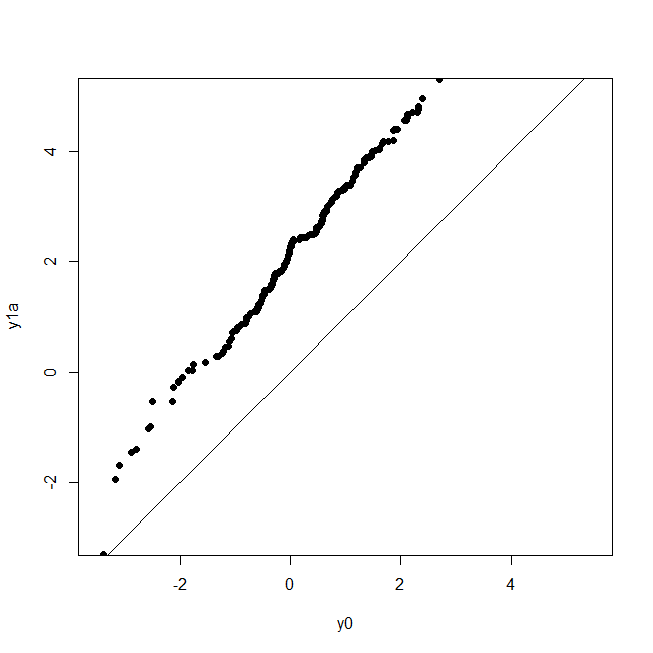
\includegraphics[height=\textheight]{images/qqplot1}}
\only<2>{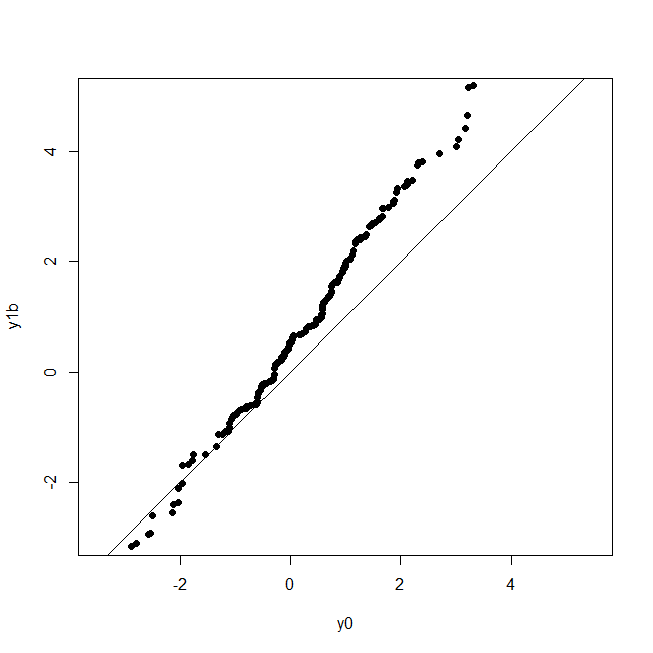
\includegraphics[height=\textheight]{images/qqplot2}}
\end{center}

}

\begin{frame}[fragile]

\frametitle{Equality of Variance tests}

\footnotesize

\begin{verbatim}
> var.test(y0, y1a)

        F test to compare two variances

data:  y0 and y1a
F = 0.60121, num df = 199, denom df = 199, 
  p-value = 0.0003635
alternative hypothesis: 
  true ratio of variances is not equal to 1
95 percent confidence interval:
 0.4549900 0.7944289
sample estimates:
ratio of variances 
         0.6012131 
\end{verbatim}

\end{frame}

\begin{frame}[fragile]

\frametitle{Equality of Variance tests}

\footnotesize

\begin{verbatim}
> var.test(y0, y1b)

        F test to compare two variances

data:  y0 and y1b
F = 0.53483, num df = 199, denom df = 199,
  p-value = 1.224e-05
alternative hypothesis:
  true ratio of variances is not equal to 1
95 percent confidence interval:
 0.4047531 0.7067133
sample estimates:
ratio of variances 
         0.5348312
\end{verbatim}

\end{frame}


\questions


\frame{\frametitle{Regression Estimation}}

\frame{

\frametitle{{\normalsize Aside: Regression Adjustment in Experiments, Generally}}

\begin{itemize}\itemsep0.5em
\item Recall the general advice that we do not need covariates in the regression to ``control'' for omitted variables (because there are none)
\item Including covariates can reduce variance of our SATE by explaining more of the variation in $Y$
\end{itemize}

}

\frame{

\frametitle{Scenario}

Imagine two regression models. Which is correct?

\begin{enumerate}
\item Mean-difference estimate of SATE is ``not significant''
\item Regression estimate of SATE, controlling for sex, age, and education, is ``significant''
\end{enumerate}

\onslide<2->{This is a small-sample dynamic, so make these decisions pre-analysis!}

}

\frame{

\frametitle{{\normalsize Treatment-Covariate Interactions}}

\normalsize

\begin{itemize}
\item The regression paradigm allows us to estimate CATEs using interaction terms
	\begin{itemize}
	\item $X$ is an indicator for treatment
	\item $M$ is an indicator for possible moderator
	\end{itemize}
\item<2-> SATE: $Y = \beta_0 + \beta_1 X + e$
\item<3-> CATEs: $$Y = \beta_0 + \beta_1 X + \beta_2 M + \beta_3 X*M + e$$
	\begin{itemize}
	\item<4-> Homogeneity: $\beta_3 = 0$
	\item<4-> Heterogeneity: $\beta_3 \neq 0$
	\end{itemize}

\end{itemize}

}

\frame{

\frametitle{Considerations}

\small

\begin{itemize}
\item<2-> Coefficients on moderators have no causal interpretation without further conditioning on observables
\item<3-> Nearly unlimited potential moderators
	\begin{itemize}
	\item First-order interactions with every covariate in dataset
	\item Second-, third-order, etc. interactions
	\end{itemize}
\item<3-> Thus, multiple comparisons problem!
\item<4-> Power (esp. if $M$ is continuous)
\end{itemize}

}




\questions


\frame{
\frametitle{BART}

\small
\begin{itemize}\itemsep0.5em
\item Estimate CATEs in a fully automated fashion
\item<2-> ``Bayesian Additive Regression Trees''
	\begin{itemize}
	\item Essentially an ensemble machine learning method
	\end{itemize}
\item<3-> Iteratively split a sample into more and more homogeneous groups until some threshold is reached using binary (cutpoint) decisions
\item<3-> Repeat this a bunch of times, aggregating across results
\end{itemize}
}

\frame{
\begin{center}
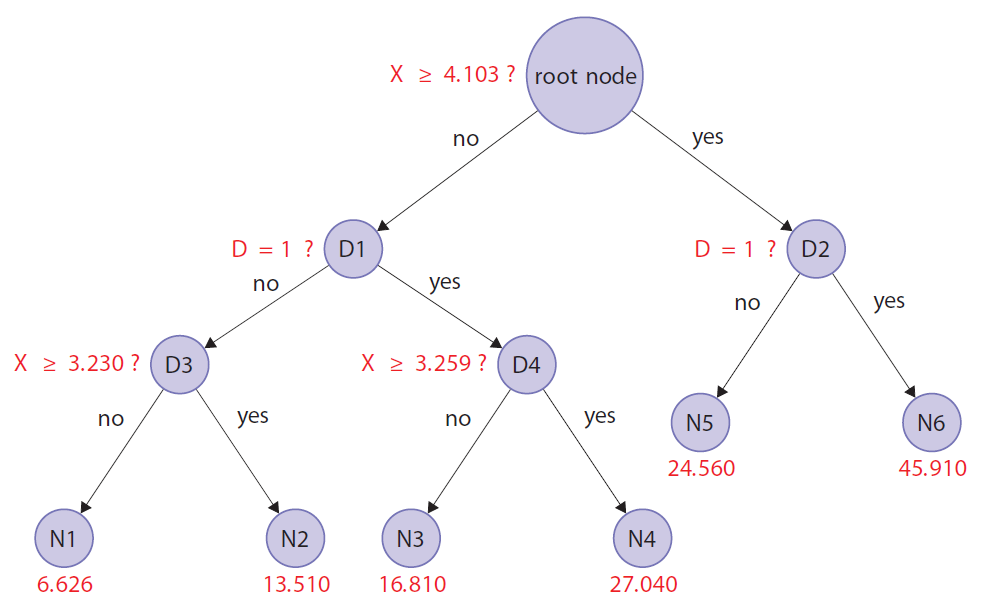
\includegraphics[width=\textwidth]{images/greenkern1}
\end{center}
{\footnotesize Green \& Kern. 2012. ``Modeling Heterogeneous Treatment Effects in Survey Experiments with Bayesian Additive Regression Trees.'' \textit{Public Opinion Quarterly} 76(3): 491--511.\par}
}

\frame{
\begin{center}
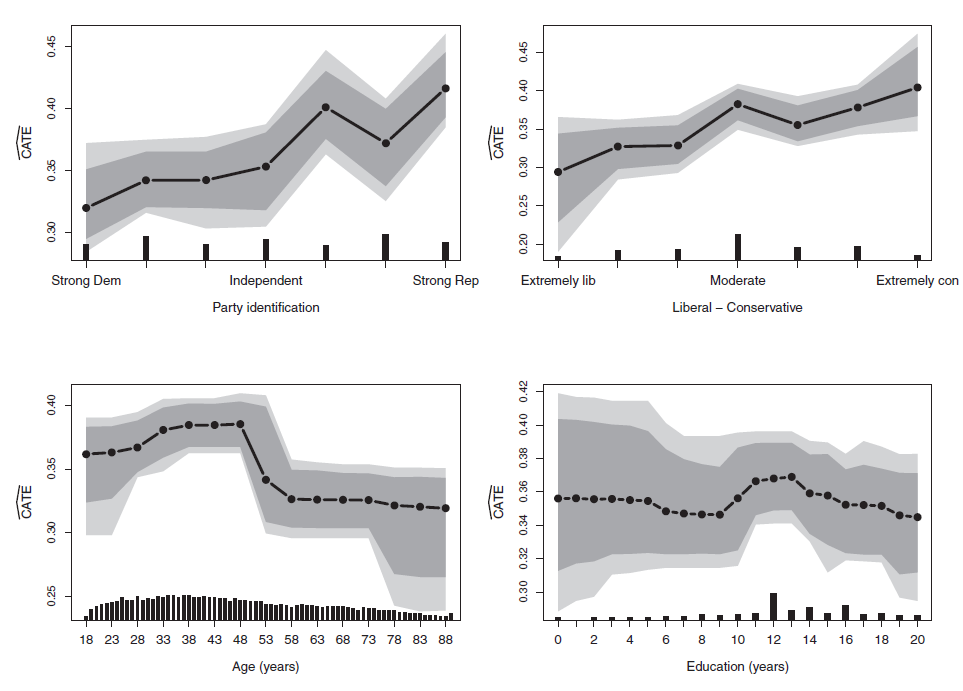
\includegraphics[height=.85\textheight]{images/greenkern2}
\end{center}
}


\frame{
\frametitle{Considerations}

\begin{itemize}\itemsep0.5em
\item BART is totally automated, conditional on the set of covariates used
\item Only really works with dichotomous covariates
\item Not widely used or tested
\item Totally post-hoc and atheoretical
\end{itemize}

}


\frame{}

\frame{

\frametitle{Replication!}

\small

\begin{itemize}\itemsep0.5em
\item If we think effects are homogeneous (across SUTO), then replications in other SUTO conditions should provide us the same SATE (within sampling error)
\item If we think effects are heterogeneous, then replications should give \textit{systematically} different SATE (or CATE) estimates
	\begin{itemize}\footnotesize
	\item<2-> Identify those patterns of heterogeneity using meta-analysis
	\item<3-> Regress effect estimates from multiple studies on SUTO features of each study
	\end{itemize}
\end{itemize}

}

\frame{}


\frame{

\frametitle{Conclusion}

\begin{itemize}\itemsep0.5em
\item Do we want to know SATE, CATE(s), or both?
\item<2-> Decide in advance
	\begin{itemize}
	\item Include in protocol
	\item Design study to estimate CATE(s)
	\end{itemize}
\item<3-> Estimation of CATEs
	\begin{itemize}
	\item Block randomization
	\item Post-hoc procedures
	\end{itemize}
\end{itemize}

}


\questions




\appendix
\frame{}

\section{Satisficing}


\frame[label=satisficing]{
\frametitle{Apparent Satisficing}
\begin{itemize}\itemsep0.5em
\item Some common measures:
	\begin{itemize}
	\item ``Straightlining''
	\item Non-differentiation
	\item Acquiescence
	\item Nonresponse
	\item DK responding
	\item Speeding
	\end{itemize}
\item Difficult to detect and distinguish from ``real'' responses
\end{itemize}
}

\frame{
\frametitle{Metadata/Paradata}
\begin{itemize}\itemsep1em
\item<1-> Timing
	\begin{itemize}
	\item Some survey tools will allow you to time page
	\item Make a prior rules about dropping participants for speeding
	\end{itemize}
\item<2-> Mousetracking or eyetracking
	\begin{itemize}
	\item Mousetracking is unobtrusive
	\item Eyetracking requires participants opt-in
	\end{itemize}
\item<3-> Record focus/blur browser events
\end{itemize}
}

\frame{
\frametitle{Direct Measures}
\begin{itemize}\itemsep1em
\item How closely have you been paying attention to what the questions on this survey actually mean?
\item<2-> While taking this survey, did you engage in any of the following behaviors? Please check all that apply.
	\begin{itemize}
	\item Use your mobile phone
	\item Browse the internet
	\item \dots
	\end{itemize}
\end{itemize}
}



\frame{
\frametitle{{\normalsize Instructional Manipulation Check}}

\small

\only<2>{Do you agree or disagree with the decision to send British forces to fight ISIL in Syria? }We would like to know if you are reading the questions on this survey. If you are reading carefully, please ignore this question, do not select any answer below, and click ``next'' to proceed with the survey.\\

\vspace{0.5em}

\footnotesize
Strongly disagree\\
Somewhat disagree\\
Neither agree nor disagree\\
Somewhat agree\\
Strongly agree\\

\vspace{1em}
\only<2>{\hyperlink{exclusion}{\beamerbutton{Return}}}
}




\end{document}
